%!TeX root=../Main Document/Dissertation.tex

\section{Appendix: Boid Graphs}

This can be seen visually represented in Fig.\ref{fig:cohesion}. It displays the cohesion force increasing as a boid moved away from the local flock centre.
\begin{figure}[H]
	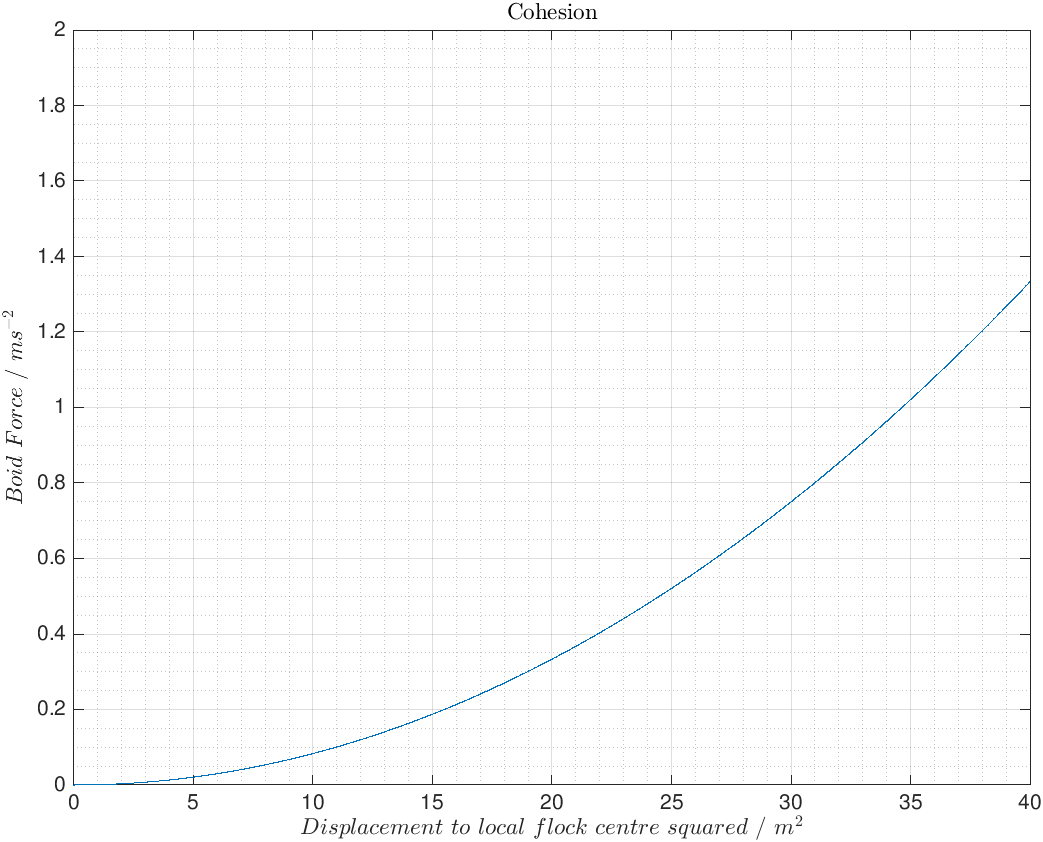
\includegraphics[width=\linewidth]{../Images/cohesion.png}
	\caption{A Graph Displaying the Cohesion Boid Force}
	\label{fig:cohesion}
\end{figure}

This can be seen visually represented in Fig.\ref{fig:alignment}. It displays the alignment force increasing as a boid moved closer to the local flock centre.
\begin{figure}[H]
	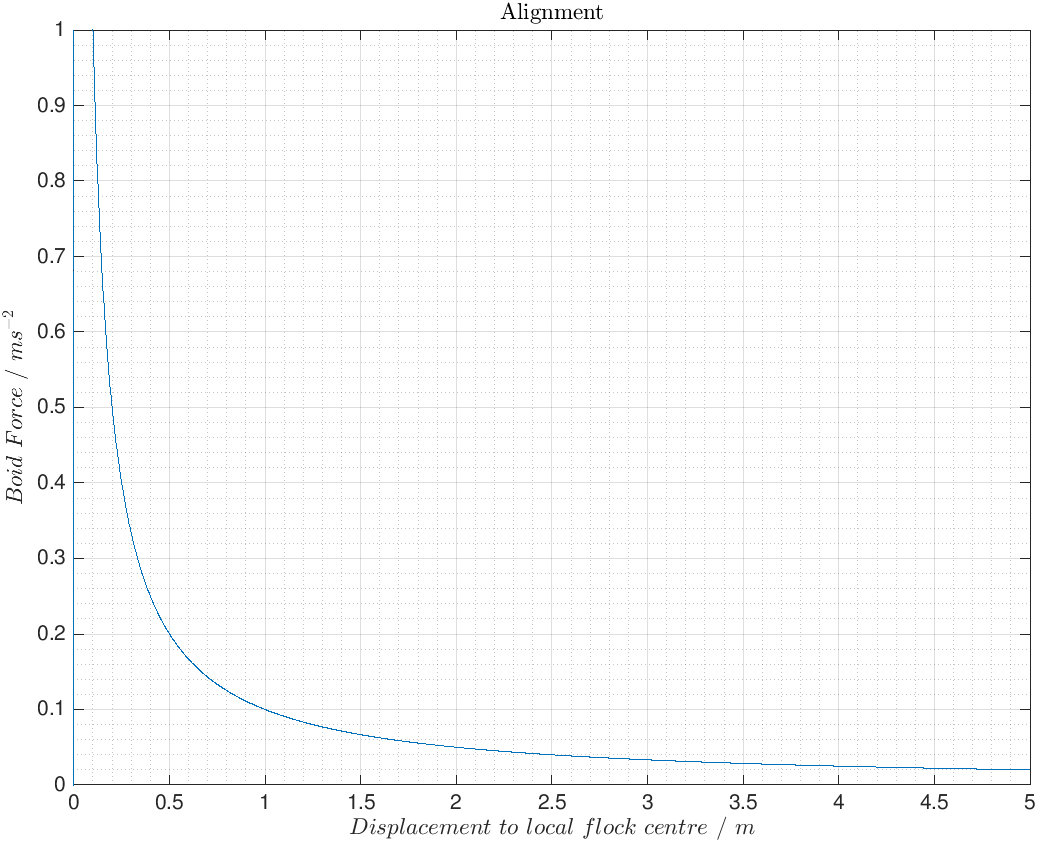
\includegraphics[width=\linewidth]{../Images/alignment.png}
	\caption{A Graph Displaying the Alignment Boid Force}
	\label{fig:alignment}
\end{figure}

This can be seen visually represented in Fig.\ref{fig:separation}. It displays the separation force increasing as the displacement between the nearest flock member and itself decreased. This separation force increased for each neighbouring boid.
\begin{figure}[H]
	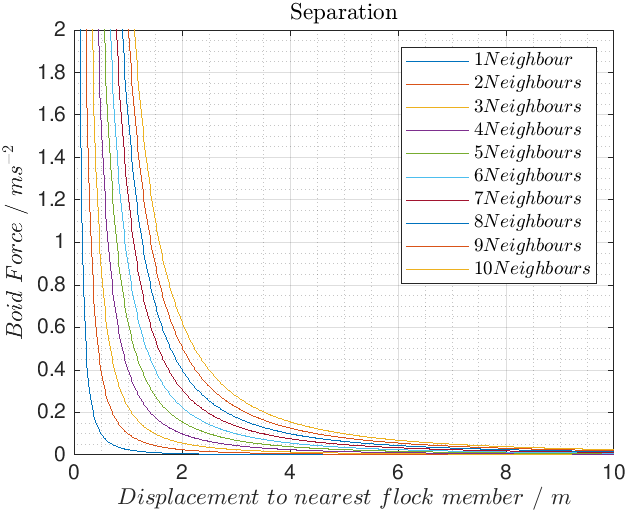
\includegraphics[width=\linewidth]{../Images/separation.png}
	\caption{A Graph Displaying the Separation Boid Force}
	\label{fig:separation}
\end{figure}

This can be seen visually represented in Fig.\ref{fig:foodattraction}. It displays relationship the food attraction force has to the displacement squared of the food resource to the boid. It represents two increases in the food attraction force and a minima inbetween, where the food attraction force decreases as the boid gets near to it, but then switches to an increase past a certain point.
\begin{figure}[H]
	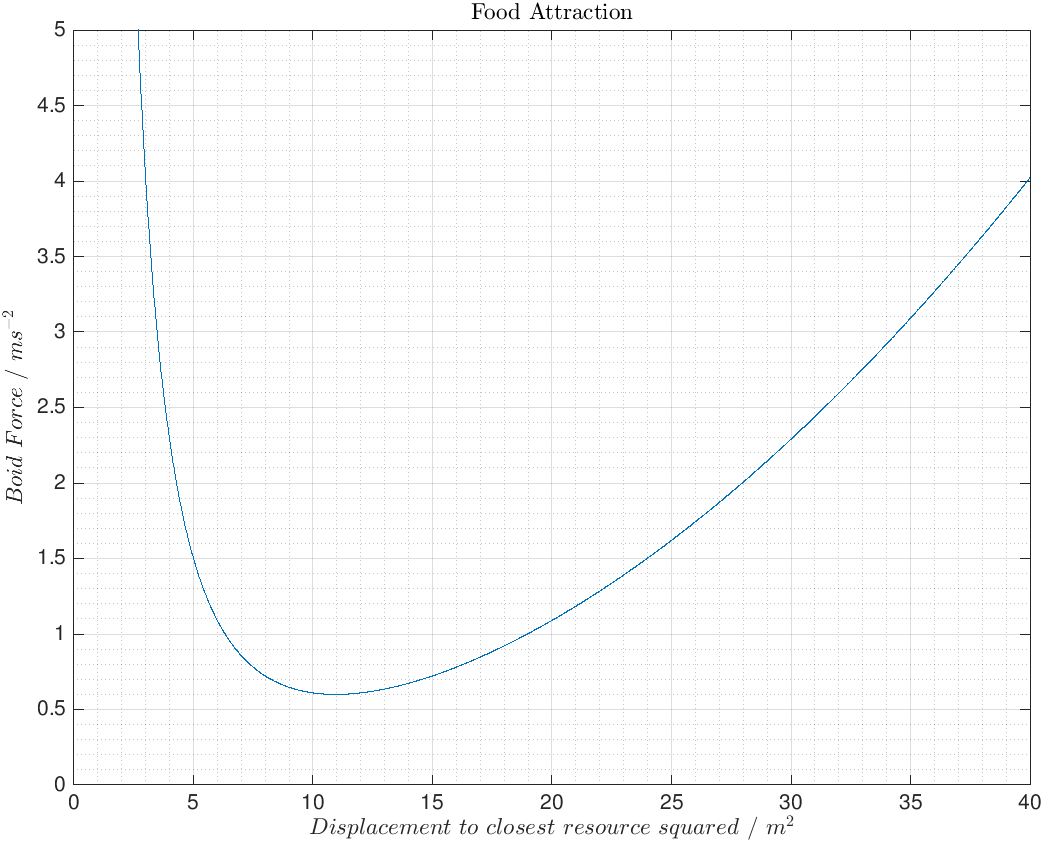
\includegraphics[width=\linewidth]{../Images/foodattraction.png}
	\caption{A Graph Displaying the Food Attraction Boid Force}
	\label{fig:foodattraction}
\end{figure}

This can be seen visually represented in Fig.\ref{fig:flockavoidance}. It displays the flock avoidance force increasing as a boid moved closer to the local flock centre.
\begin{figure}[H]
	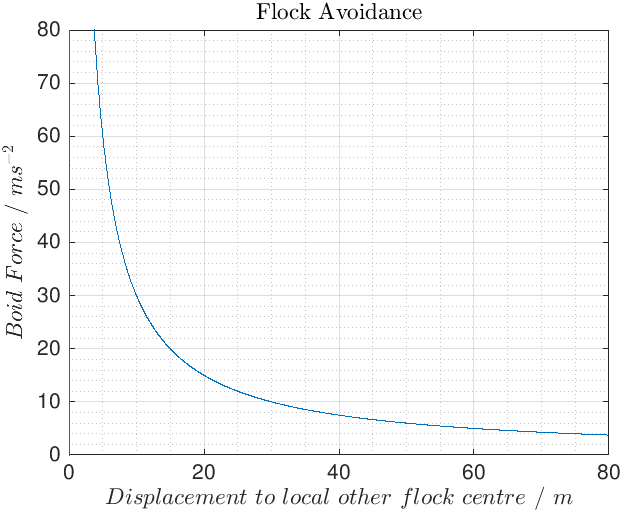
\includegraphics[width=\linewidth]{../Images/flockavoidance.png}
	\caption{A Graph Displaying the Flock Avoidance Boid Force}
	\label{fig:flockavoidance}
\end{figure}











